\documentclass[a4paper,twoside,12pt]{article}
\usepackage{amsmath}
\usepackage{amsfonts}
\usepackage{amssymb}
\usepackage[utf8]{inputenc}
\usepackage[T1]{fontenc}
\usepackage{fancyhdr}
\usepackage{stmaryrd}
\usepackage{textcomp}
\usepackage[french]{babel}
\usepackage{variations}
\usepackage{graphicx}
\usepackage{array}
\usepackage{arydshln}
\usepackage{verbatim}
\usepackage{psfrag}
\usepackage{bbm}
\usepackage{ifthen}

\newlength{\myhoffset}
\newlength{\mytextwidth}
\newlength{\myvoffset}
\newlength{\mytextheight}
\setlength{\myhoffset}{-1cm}
\setlength{\mytextwidth}{2.5cm}
\setlength{\myvoffset}{-2.5cm}
\setlength{\mytextheight}{3cm}

\addtolength{\hoffset}{\myhoffset}
\addtolength{\textwidth}{\mytextwidth} 
\addtolength{\voffset}{\myvoffset}
\addtolength{\textheight}{\mytextheight} 

%textpos : permet de placer des éléments par leur coordonnées absolues sur la page
% utilisé pour les entêtes et pied de pages

\usepackage[absolute]{textpos}
\setlength{\TPHorizModule}{1mm}
\setlength{\TPVertModule}{\TPHorizModule}
\textblockorigin{-\myhoffset}{-\myvoffset}

% fancyhdr : permet de personnaliser les entêtes et pieds de page des documents

\usepackage{fancyhdr}

%% pdfpages : utilisé pour insérer la page de garde avant le document

\usepackage{pdfpages}

\setlength\parindent{0pt}

\linespread{1.1}


%%%% debut macro %%%%
\makeatletter
\def\hlinewd#1{%
\noalign{\ifnum0=`}\fi\hrule \@height #1 %
\futurelet\reserved@a\@xhline}
\makeatother
%%%% fin macro %%%%

\newcounter{partie}
\newcounter{sous-partie}

\renewcommand{\thesection}{\Roman{section}}

\newenvironment{partie}[1]
{
\section{#1}
}
{

}

\newcommand{\mymark}[1]{\markboth{\MakeUppercase{#1}}{\MakeUppercase{#1}}}

\newenvironment{biblio}
{
\section*{Bibliographie}
\addcontentsline{toc}{section}{Bibliographie}
\mymark{Bibliographie}
}
{

}

\newenvironment{intro}
{
\section*{Introduction}
\addcontentsline{toc}{section}{Introduction}
\mymark{Introduction}
}
{

}

\newenvironment{remerciements}
{
\section*{Remerciements}
\addcontentsline{toc}{section}{Remerciements}
\mymark{Remerciements}
}
{

}


\newenvironment{sous-partie}[1]
{
\subsection{#1}
}
{

}



% Divers

% Permet de faire des cadres dans le document
\newcommand{\cadre}[1]{\renewcommand{\arraystretch}{0.4}\begin{array}{|c|}\hline\\#1\\\\\hline\end{array}}
\newcommand{\cadret}[1]{\renewcommand{\arraystretch}{0.4}\begin{tabular}{|c|}\hline\\#1\\\\\hline\end{tabular}}
\newcommand{\semicadre}[1]{\renewcommand{\arraystretch}{0.3}\begin{array}{c|}#1\\\\\hline\end{array}}

% Commandes mathématiques

\newcommand{\equivalent}[2]{\!\!\renewcommand{\arraystretch}{1}\begin{array}[t]{c}\Huge\sim\\^{#1\rightarrow#2}\end{array}\!\!}
\newcommand{\tend}[2]{\!\renewcommand{\arraystretch}{1}\begin{array}[t]{c}-\!-\!\!\!\longrightarrow\\^{#1\rightarrow#2} \\ [-1.5ex]\end{array}\!}
\newcommand{\egal}[2]{\!\!\renewcommand{\arraystretch}{1}\begin{array}[t]{c}=\\^{#1\rightarrow#2}\end{array}\!\!}
\newcommand{\fin}{\vspace{0.2cm}\\}
\newcommand{\finq}{\vspace{0.5cm}\\}
\newcommand{\sh}{\mathrm{sh}\,}
\newcommand{\abs}[1]{\left\vert#1\right\vert }
\newcommand{\ch}{\mathrm{ch}\,}

\renewcommand{\o}[1]{\mathrm{o}\!\left(#1\right)}
\newcommand{\etoile}{\hspace*{1cm}$\star$\hspace*{0.5cm}}
\renewcommand{\th}{\mathrm{th}\,}
\renewcommand{\arcsin}{\mathrm{Arcsin}\,}
\renewcommand{\arccos}{\mathrm{Arccos}\,}
\newcommand{\argsh}{\mathrm{Argsh}\,}
\newcommand{\argch}{\mathrm{Argch}\,}
\newcommand{\argth}{\mathrm{Argth}\,}
\newcommand{\rg}{\mathrm{rg}\,}
\renewcommand{\arctan}{\mathrm{Arctan}\,}
\newcommand{\sq}{\hspace*{1.4cm}\stepcounter{sq}(\alph{sq})\hspace*{0.5cm}}
\newcommand{\rcl}{\begin{array}{rcl}}
\newcommand{\ea}{\end{array}}
\newcommand{\str}[1]{\renewcommand{\arraystretch}{#1}}
\renewcommand{\tfrac}[2]{\textstyle\frac{#1}{#2}}
\newcommand{\Cl}[1]{$C^{#1}$}
\newcommand{\mathCl}[1]{C^{#1}}
\renewcommand{\t}[1]{\tilde{#1}}
\renewcommand{\l}{\lambda}
\newcommand{\ds}{\displaystyle}
\newcommand{\R}{\mathbb{R}}
\newcommand{\C}{\mathbb{C}}
\newcommand{\Q}{\mathbb{Q}}
\newcommand{\Z}{\mathbb{Z}}
\newcommand{\N}{\mathbb{N}}
\newcommand{\Ker}{\mathrm{Ker}\,}
\newcommand{\Vect}{\mathrm{Vect}}
\renewcommand{\lvert}{\left\vert}
\renewcommand{\Im}{\mathrm{Im}\,}
\renewcommand{\rvert}{\right\vert}
\newcommand{\mnk}{\mathcal{M}_n(K)}
\newcommand{\mnc}{\mathcal{M}_n(C)}
\newcommand{\ppcm}{\mathrm{ppcm}}
\newcommand{\Tr}{\mathrm{Tr}\,}
\renewcommand{\t}[1]{^t\!#1}
\newcommand{\scal}[2]{\left\langle #1|#2\right\rangle}
\newcommand{\scalindice}[4]{\phantom{\langle}_{#3}\!\left\langle #1|#2\right\rangle_{#4}}
\newcommand{\p}[1]{\left( #1 \right)}
\newcommand{\crochet}[1]{\left[ #1 \right]}
\newcommand{\nr}[1]{\left\|\,#1\,\right\|}
\newcommand{\tab}{\hspace*{1cm}}

\newcommand{\esp}[1]{\mathbb{E}\!\crochet{#1}}
\newcommand{\espcond}[2]{\mathbb{E}_{#1}\!\crochet{#2}}

\renewcommand{\P}[1]{\mathbb{P}\!\p{#1}}
\newcommand{\Pcond}[2]{\mathbb{P}_{#1}\!\p{#2}}

\renewcommand{\binom}[2]{\left(\begin{array}{c}#1\\#2\end{array}\right)}

\newcommand{\car}[1]{\mathbf{1}_{#1}}

\newcommand{\matdd}[4]{\left({\begin{array}{cc} #1 & #2\\ #3 & #4 \ea}\right)\vspace{0.05cm}}

\newcommand{\supp}[1]{\text{supp}\left(#1\right)}

\renewcommand{\ge}{\geqslant}
\renewcommand{\le}{\leqslant}

\newcommand{\lebesgue}{\mathcal{L}}

\newcommand{\Drond}{\mathcal{D}}

\renewcommand{\Re}{\mathcal{R}e}
\newcommand{\obs}[1]{\hat{#1}}
\newcommand{\ket}[1]{\vert #1 \rangle}
\newcommand{\bra}[1]{\langle #1 \vert}
\newcommand{\braindice}[2]{\!\phantom{\langle}_{#2}\!\left\langle #1\right\vert}

\newcommand{\prodscal}[2]{\left\langle#1,#2\right\rangle}

\newcommand{\vect}[2]{\left(\str{1}\begin{array}{cc}#1 & #2 \ea\right)}
\newcommand{\vecttrans}[2]{\left(\str{1}\begin{array}{c}#1 \\ #2 \ea\right)}

\renewcommand{\v}[1]{\underline{#1}}

\newcommand{\Dp}[2]{\dfrac{\partial #1}{\partial #2}}
\newcommand{\grad}{\mathrm{grad}\,}
\newcommand{\vgrad}{\v{\mathrm{grad}}\,}


\pagestyle{fancy}

\setlength{\headheight}{2cm}

\renewcommand{\headrulewidth}{0.4pt}
\renewcommand{\footrulewidth}{0pt}

\fancyhead{}
\fancyfoot{}

\fancyhead[R]{
\includegraphics[height=1.5cm]{./images/Charte_graphique_polytechnique/logo_x_simple.png}}

\fancyfoot[RE,LO]{\thepage}
\fancyhead[L]{\leftmark}


\begin{document}
\setlength{\hoffset}{0cm}
\setlength{\voffset}{0cm}

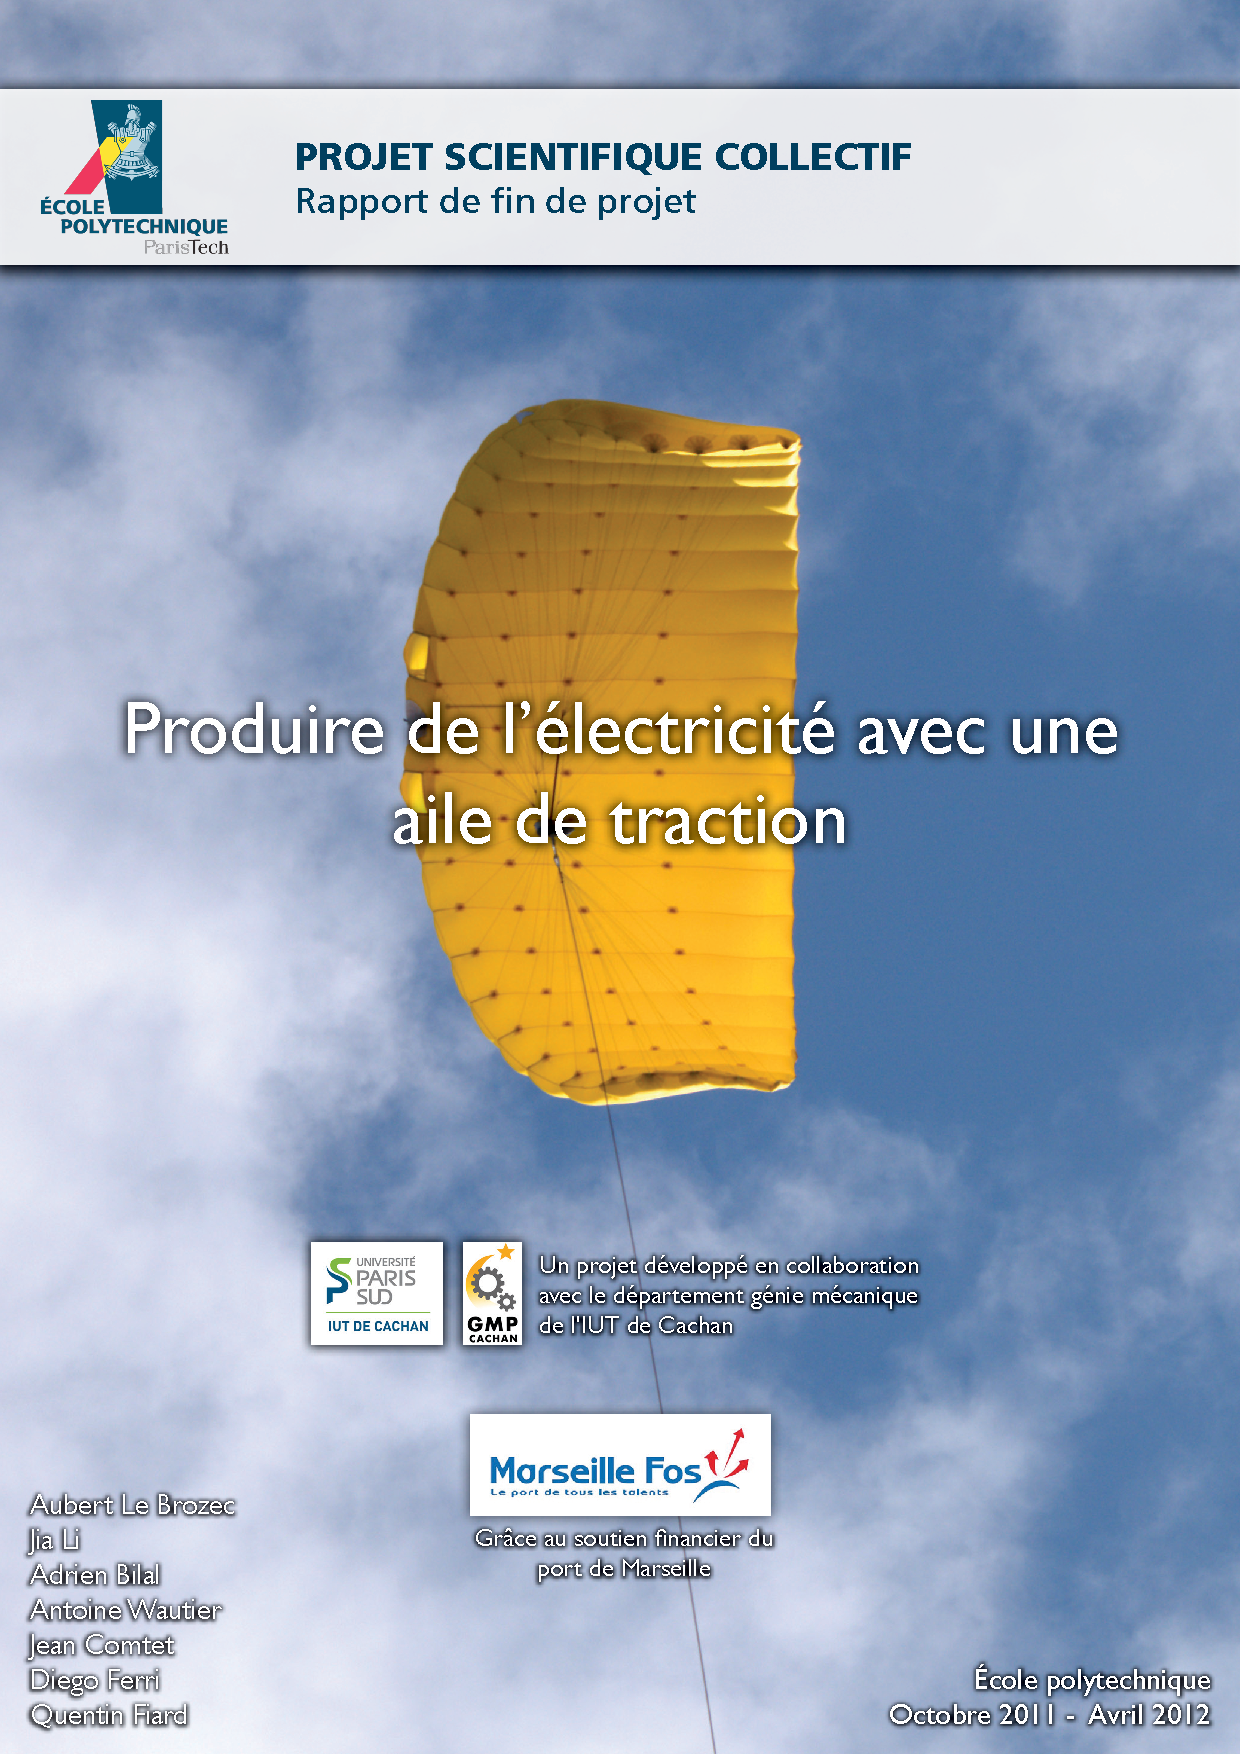
\includepdf{./images/page_de_garde.pdf}

\setlength{\hoffset}{\myhoffset}
\setlength{\voffset}{\myvoffset}

\newpage

\tableofcontents

\newpage

\begin{intro}
- poser le problème
- le problème en grandeur nature
- ce qui a déja été fait sur le sujet
- qques chiffres sur les cargos...
- approche énergétique
- insister sur le fait que c'est en plein boom
\end{intro}

\newpage

\begin{remerciements}

\end{remerciements}

\newpage



\begin{partie}{Physique de l'aile}

Modélisation du pb , notations, hypothèses (voile rigide, fils tendus et droits, bord d’attaque perp à la trajectoire)

\begin{sous-partie}{Modèle 2D}

\end{sous-partie}

\begin{sous-partie}{Étude qualitative de la dynamique (2D puis en se donnant une trajectoire)}

\end{sous-partie}

\begin{sous-partie}{Gerris, calcul des tables des coefficients aéro}

\end{sous-partie}

\end{partie}

\newpage

\begin{partie}{Description technique de l'expérience}

\begin{sous-partie}{Comment passer du problème réel au problème réduit ?}
- cargo + centrale : notre exp s'applique aux 2
\newline
- le boitier dont on étudie la conception sera en fait en l'air
\newline
- analyse de la similitude des écoulements
\newline
- dimensionnement

\end{sous-partie}

\begin{sous-partie}{Cahier des charges}
- quelles grandeurs doit on mesurer ? %NL%
quelle précision ?
\\
- quelle vitesse de moteur ? %NL%
quelle précision ? %NL%
quel couple ?
\\
- quelle force va s'appliquer sur le système ? %NL%
quelle robustesse prévoir ?
\end{sous-partie}

\begin{sous-partie}{Solutions apportées}
- partie électronique : circuits intégrés, capteurs, contrôle du moteur
\\
- partie mécanique :  moteur, anémomètre, prototypage rapide IUT Cachan, échec de l'AX-18, travail du bois, caméra...
\end{sous-partie}

\begin{sous-partie}{Démarches}
- IUT Cachan
\\
- Sponsor Port de Marseille, création d'un binet, plaquette sponsors
\\
- concours energia
\end{sous-partie}




\end{partie}

\newpage

\begin{partie}{Contrôle numérique du système}
Intro (ou dans III.2) : schéma d'asservissement pour rappeler quelles grandeurs on commande, quelles grandeurs on mesure + schéma couche par  couche comme dans la thèse

\begin{sous-partie}{Description de l'architeture informatique globale}
- schéma
\\
- préciser le contrôle du moteur, des capteurs (programme caméra)
\end{sous-partie}
\begin{sous-partie}{Calcul des coéfficients aérodynamiques via Gerris}

\end{sous-partie}

\begin{sous-partie}{Description théorique de l'asservissement}
La trajectoire en 8 que nous souhaitons faire suivre à notre aile de traction-trajectoire que nous avons nous-mêmes déterminée à l'aide d'un algorithme d'optimisation comme on pourra le voir en partie IV- n'est pas une trajectoire auto-stable : sans contrôle, l'aile de Kite surf ne peut rester dessus. Il y a donc besoin d'un contrôle en permanence au niveau de la longueur des câbles pour que l'aile puisse suivre cette trajectoire. 
\newline
Par ailleurs, on ne peut enregistrer une séquence d'asservissement en avance pour l'imposer ensuite à l'aile. En effet, les vents étant relativement changeants, les commandes que l'on donne à l'aile doivent être adaptées au conditions climatiques à tout instant.
\newline
C'est pourquoi un asservissement en temps réel de la position de l'aile est indispensable.
Rappelons que nous considérons dans cette étude que l'aile vole sur une sphère de rayon r fixé ($r=20m$ pour notre expérience, $R=600 m$ pour les systèmes d'ailes de traction sur cargos) et que nous connaissons la position de l'aile grâce aux mesures des angles $\theta$ et $\phi$ (via des capteurs incrémentaux au niveau de la liaison de l'aile avec le sol) ainsi que son orientation décrite par les angles $\psi_1$ et $\psi_2$ (l'angle  $\psi_1$ est connu directement à partir du différentiel de longueur entre les 2 brins, et $\psi_2$ est obtenu à l'aide de traitement d'image par caméra).
Par ailleurs, nous disposons également des dérivées de ces 4 grandeurs en calculant des taux d'accroissement à intervalles de temps petits (suffisamment petits pour que l'incertitude due à ces calculs ne soit pas dominante, comme on l'explique dans la suite). En pratique, comme nous allons le voir dans la suite, nous n'avons pas besoin de connaître les grandeurs $\dot{\psi_1}(t)$ et $\dot{\psi_2}(t)$ pour l'asservissement.
\newline
La fonction d'état du Kite s'écrit alors :
$$X(t)=(\theta(t),\phi(t),\dot{\theta}(t),\dot{\phi}(t),\psi_1(t), \psi_2(t))^T$$
Il faut à présent définir le contrôle $u$ que l'on a sur le système. Expérimentalement, nous avons pu constater le fait qu'il est possible de faire faire des 8 bouclés au Kite en agissant uniquement sur le différentiel de longueur entre les 2 brins. Nous prenons donc pour grandeur de contrôle u la grandeur $\dot{\psi_1}(t)$ qui est directement reliée au différentiel de vitesse entre les deux brins et donc à la vitesse de rotation du moteur.
\newline
\begin{huge}
Insérer schéma Aubert 1 
\end{huge}
(et introduire les grandeurs x et L)
\newline
Comme $L x \cos \psi_1(t) = l_1 l_2 -r^2 +\frac{L^2}{4}$ alors : $$\psi_1(t) \approx \arccos \big[\frac{1}{2} + \frac{2(l_1 l_2-r^2)}{L^2}\big]-\pi$$ donc
$$u = \dot{\psi_1}(t)= -\frac{2\frac{d}{dt}[l_1(t) l_2(t)]}{L^2}* \frac{1}{1/2}$$ car $$1-(\frac{1}{2} + \frac{2(l_1 l_2-r^2)}{L^2})^2 = 1-\frac{1}{4} - 2 \frac{l_1(t)l_2(t)}{L^2} + \big(4 \frac{l_1(t)l_2(t)}{L^2}\big)^2 \approx \frac{3}{4}-\frac{1}{2} + \frac{1}{4}= \frac{1}{2}$$
On calcule : $\frac{d}{dt}[l_1(t) l_2(t)] = (\dot{l_1}(t)+ \dot{l_2}(t))\frac{l_1 + l_2}{2}+(\dot{l_1}(t)- \dot{l_2}(t))\frac{l_2 - l_1}{2}$. Comme $l_1(t)+l_2(t)=C^{te}$, on a alors $\frac{d}{dt}[l_1(t) l_2(t)]= (\dot{l_1}(t)- \dot{l_2}(t))\frac{l_2 - l_1}{2}$, d'où :
$$u =  \frac{2 (\dot{l_1}(t)-\dot{l_2}(t))(l_1(t)+l_2(t))}{L^2} \approx \frac{4 r \dot{\mathcal{M}} R_{arbre moteur}}{L^2}$$ où $\dot{\mathcal{M}}$ est la vitesse du moteur (en pratique, c'est ce que l'on contrôle directement dans l'expérience.



On définit ensuite une fonction distance qui permet de voir de combien l'aile de traction s'est éloignée de la trajectoire prévue initialement (éloignement suite à changement brutal de vent, incertitudes dans le repérage de la position, inexactitudes dans l'asservissement en temps réel...). Notons f cette fonction. Il est à noter que, si l'algorithme effectue le calcul de la commande tous les $\Delta t$ (et applique la commande précédente pendant qu'il calcule la nouvelle), l'algorithme doit minimiser f non pas en une itération, mais pendant sur  une période de temps bien choisie (appelée horizon, notée $T_H$), pour éviter les phénomènes d'oscillation décrits par la figure suivante : 
\newline
\begin{Huge}
insérer schéma 2 (oscillations)
\end{Huge}
\newline
Le principe de l'asservissement en temps direct est alors le suivant : au temps t, on calcule (à l'aide d'un algorithme d'optimisation) liste de commandes à effectuer $(u_1,u_2,...)$ qui va permettre de minimiser (sur la durée $T_H$) la distance entre la trajectoire effective du Kite, et la trajectoire à suivre. Si on calcule N commandes différentes pour le temps $T_H$, ceci signifie que le moteur va changer d'allure tous les $\frac{T_H}{N}s$ pour garder le kite sur la trajectoire. Pendant que le moteur applique ces commandes, on en calcule une nouvelle série de façon à ce que le moteur tourne en continu. Cette procédure est résumée sur le schéma suivant : 
\newline
\begin{huge}
insérer schéma 3 (pas de temps)
\end{huge}
Remarque : la durée $\delta t$ doit être choisie petite pour la précision de l'algorithme, pas trop petite non plus pour que le temps de calcul reste raisonnable et pour que le moteur ait le temps de réagir à chacune de ces modifications de sa vitesse.
\end{sous-partie}

\begin{sous-partie}{Acado et asservissement en temps réel}
Sur les conseils de Pierre Martinon (Chercheur au CMAP), nous avons utilisé le code Acado Toolkit, développé par Moritz Diehl, pour réaliser notre asservissement en temps réel, qui est un code crée spécifiquement pour ce genre de problème (Moritz Diehl a d'ailleurs étudié personnellement la producion d'énergie à l'aide d'ailes de traction).
Son collaborateur Mario Zanon a accepté de nous aider à distance en nous guidant sur le débugage de problèmes internes à Acado.

Nous allons à présent évoquer deux points : les pas de temps que nous nous sommes fixés en pratique et la précision des calculs que nous avons réalisé.


- problème de détermination de l'horizon de temps (pour être assez précis et pour que le temps de calcul ne soit pas trop long
\\
- déterminer le pas de temps de l'algo (compromis entre précision et capacités des composants physiques) + la précision à laquelle on doit faire les calculs
\end{sous-partie}


\end{partie}

\newpage

\begin{partie}{Analyse de l'expérience et élargissement}

\begin{sous-partie}{Contrôle de l'aile via joystick et via asservissement}

\end{sous-partie}

\begin{sous-partie}{Limites du modèle réduit }
Pourquoi l'expérience est difficile à réaliser
\\
- aile souple
\\
- déformation des fils
\\
- inertie du moteur
\\
- vent instable, non horizontal
\\
- imprécision de calcul des coefficients ?
\\
Pourquoi l'expérience ne cadre pas tout à fait avec le modèle réel
- similitude de l'écoulement ?
\\
- boitier qui n'est pas en l'air
\end{sous-partie}

\begin{sous-partie}{Approche énergétique}
On a vu qu'il est possible de réaliser  l'asservissement d'une aile de traction.
\\
Comment mettre ceci à profit pour avoir le plus d'énergie possible ?
\\
Trajectoires optimales, robustesse.
\end{sous-partie}

\end{partie}

\newpage

\begin{biblio}

\end{biblio}

\end{document}
